% 12 variables in here:
% u_1 = 0.0, h_1 = 9.0, U_1 = 0.0, H_1 = 10.0, u_2 = 0.0, h_2 = 10.0, U_2 = 0.0, H_2 = 10.0, u_3 = 0.0, h_3 = 10.0, U_3 = 0.0, H_3 = 10.0
\begin{figure}[h!t]
\centering
% \subfigure[] { 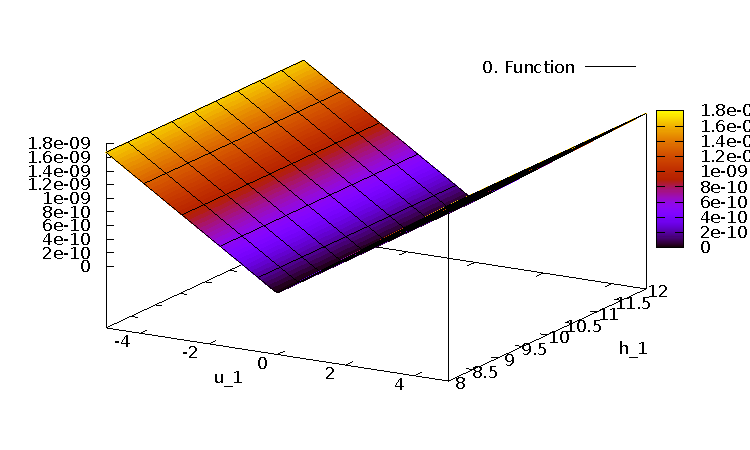
\includegraphics[scale=\zoomfactor]{{{3_punkte_1_geschwindigkeit_verringert/x_y_0.0_10.0_0.0_10.0_0.0_10.0_0.0_10.0_0.0_10.0f0}}} }
% \subfigure[] { 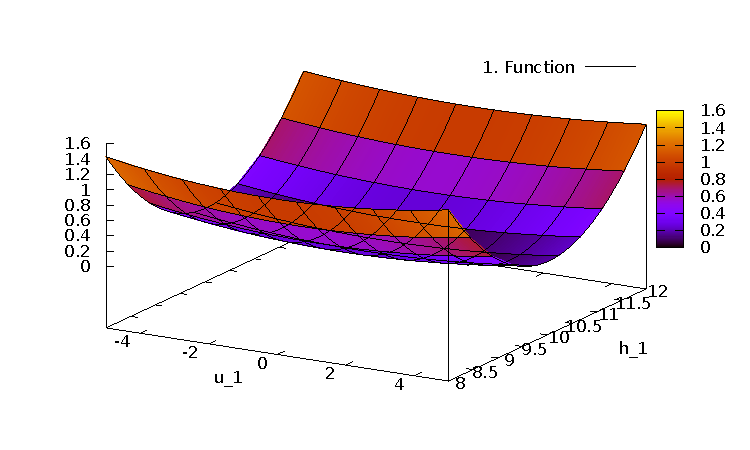
\includegraphics[scale=\zoomfactor]{{{3_punkte_1_geschwindigkeit_verringert/x_y_0.0_10.0_0.0_10.0_0.0_10.0_0.0_10.0_0.0_10.0f1}}} }

\subfigure[Height for point $p_2^L$] {
  \label{subfig:height-p1-three-points-height-verringert}
  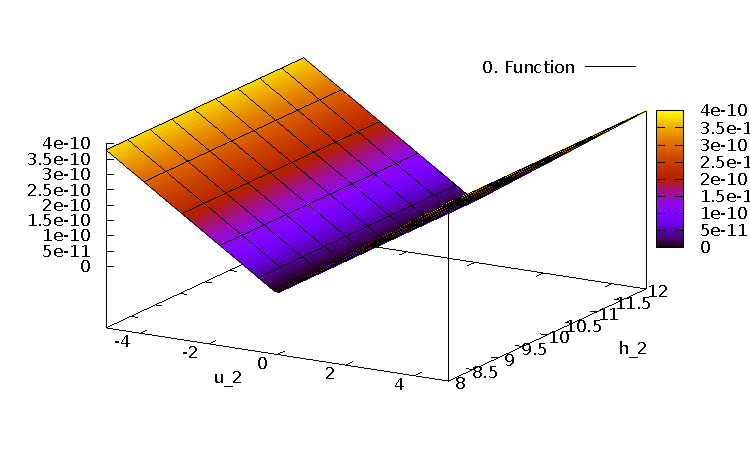
\includegraphics[scale=\zoomfactor]{{{3_punkte_1_geschwindigkeit_verringert/0.0_9.0_0.0_10.0_x_y_0.0_10.0_0.0_10.0_0.0_10.0f0}}} 
  % 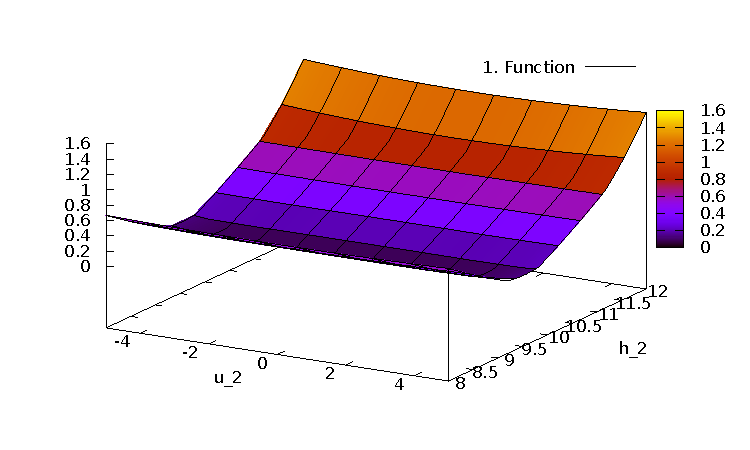
\includegraphics[scale=\zoomfactor]{{{3_punkte_1_geschwindigkeit_verringert/0.0_9.0_0.0_10.0_x_y_0.0_10.0_0.0_10.0_0.0_10.0f1}}} 
}
\subfigure[Impulse for point $p_2^L$] { 
  %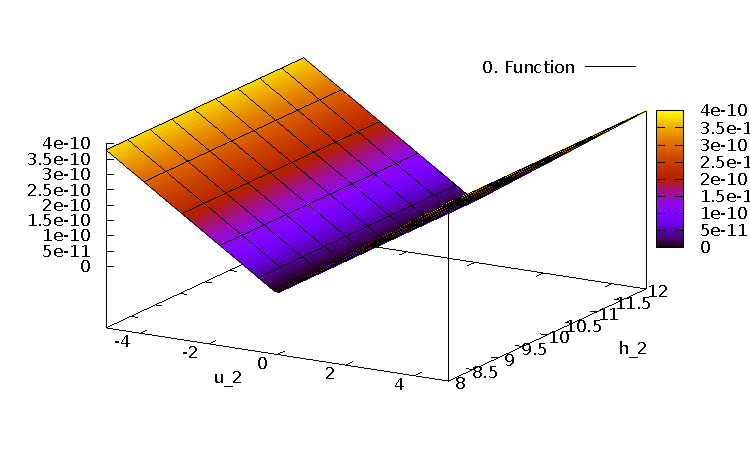
\includegraphics[scale=\zoomfactor]{{{3_punkte_1_geschwindigkeit_verringert/0.0_9.0_0.0_10.0_x_y_0.0_10.0_0.0_10.0_0.0_10.0f0}}} 
  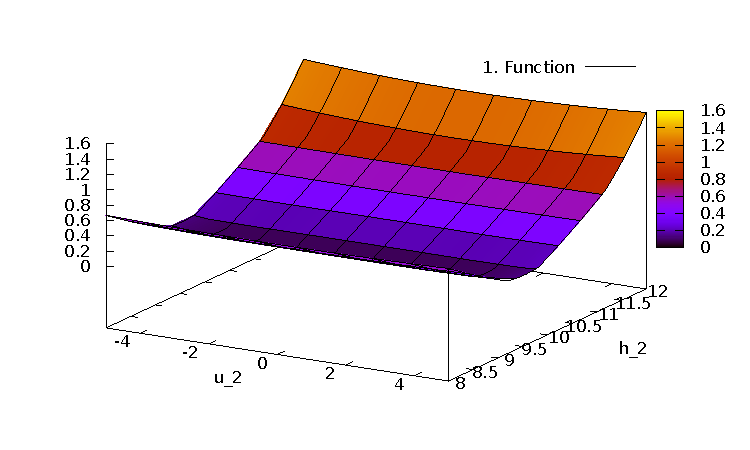
\includegraphics[scale=\zoomfactor]{{{3_punkte_1_geschwindigkeit_verringert/0.0_9.0_0.0_10.0_x_y_0.0_10.0_0.0_10.0_0.0_10.0f1}}} 
}

\subfigure[Impulse for point $p_3^L$] {
  %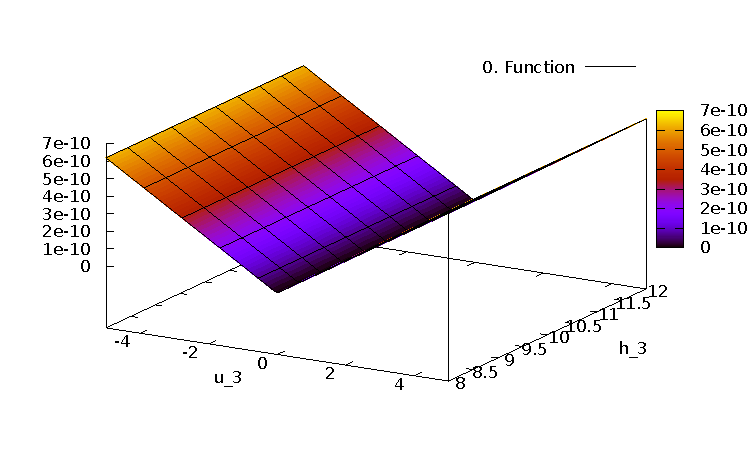
\includegraphics[scale=\zoomfactor]{{{3_punkte_1_geschwindigkeit_verringert/0.0_9.0_0.0_10.0_0.0_10.0_0.0_10.0_x_y_0.0_10.0f0}}} 
  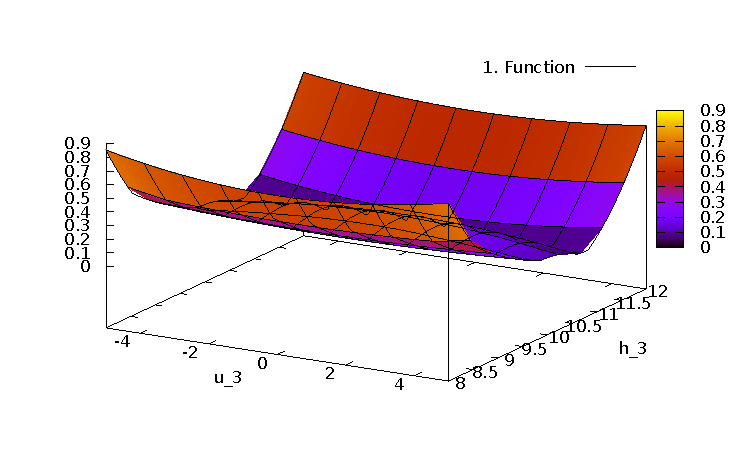
\includegraphics[scale=\zoomfactor]{{{3_punkte_1_geschwindigkeit_verringert/0.0_9.0_0.0_10.0_0.0_10.0_0.0_10.0_x_y_0.0_10.0f1}}} 
}
\subfigure[Impulse for point $p_1^R$] { 
  %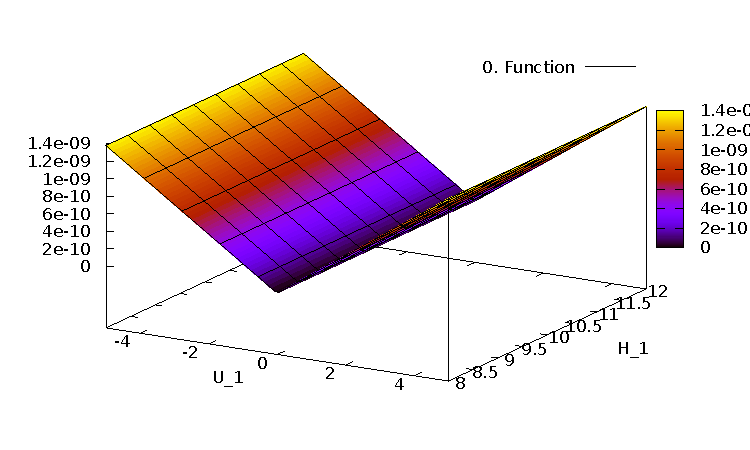
\includegraphics[scale=\zoomfactor]{{{3_punkte_1_geschwindigkeit_verringert/0.0_9.0_x_y_0.0_10.0_0.0_10.0_0.0_10.0_0.0_10.0f0}}} 
  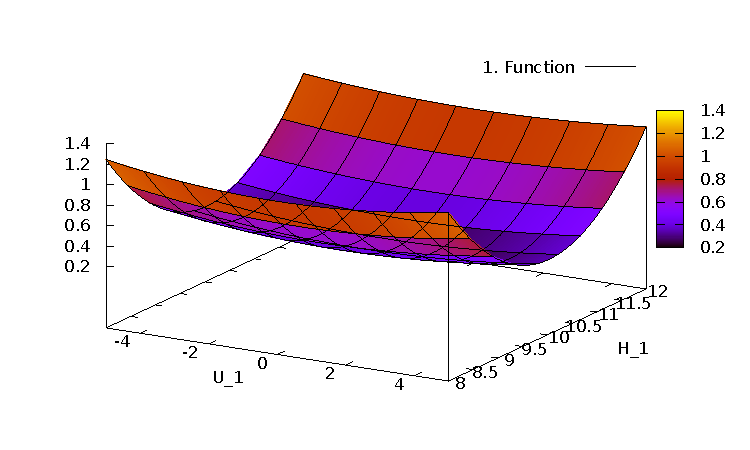
\includegraphics[scale=\zoomfactor]{{{3_punkte_1_geschwindigkeit_verringert/0.0_9.0_x_y_0.0_10.0_0.0_10.0_0.0_10.0_0.0_10.0f1}}} 
}

\subfigure[Impulse for point $p_2^R$] {
  %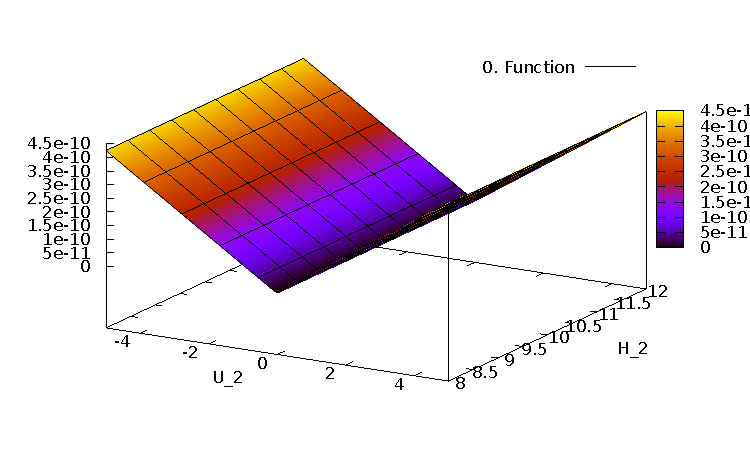
\includegraphics[scale=\zoomfactor]{{{3_punkte_1_geschwindigkeit_verringert/0.0_9.0_0.0_10.0_0.0_10.0_x_y_0.0_10.0_0.0_10.0f0}}} 
  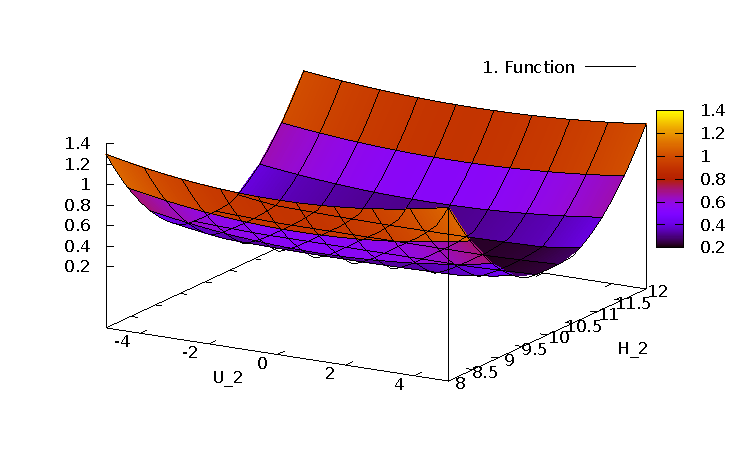
\includegraphics[scale=\zoomfactor]{{{3_punkte_1_geschwindigkeit_verringert/0.0_9.0_0.0_10.0_0.0_10.0_x_y_0.0_10.0_0.0_10.0f1}}} 
}
\subfigure[Impulse for point $p_3^R$] {
  %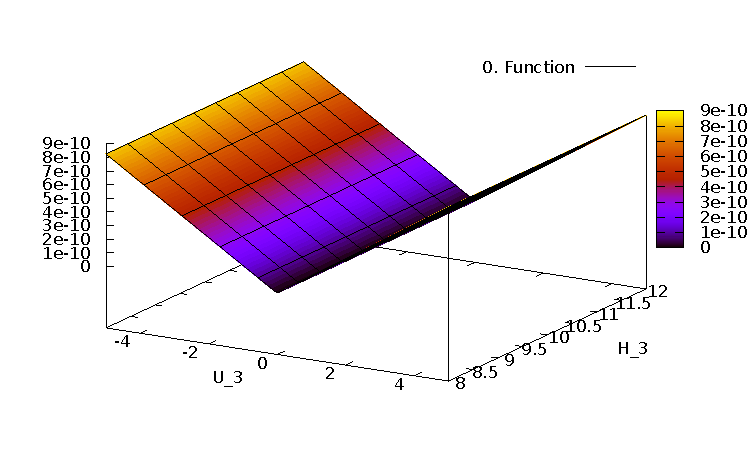
\includegraphics[scale=\zoomfactor]{{{3_punkte_1_geschwindigkeit_verringert/0.0_9.0_0.0_10.0_0.0_10.0_0.0_10.0_0.0_10.0_x_yf0}}} 
  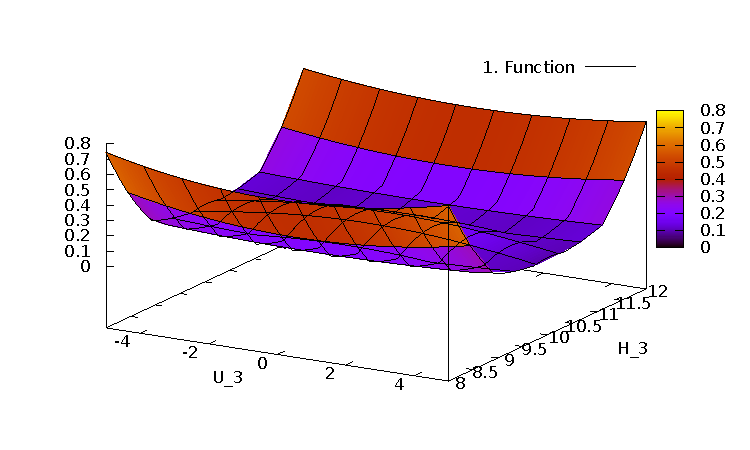
\includegraphics[scale=\zoomfactor]{{{3_punkte_1_geschwindigkeit_verringert/0.0_9.0_0.0_10.0_0.0_10.0_0.0_10.0_0.0_10.0_x_yf1}}} 
}
\caption{Three points for each triangle. All points except $p_1$ have height 10, impulse 0. Point $p_1$ is set to $(9,0)$. Since the error in the $h$-component is not very different to the one depicted in subfigure \ref{subfig:height-p1-three-points-height-verringert} (i.e.\,same shape, magnitude $10^{-15}$), we omitted the plots. Especially the plots for $p_2^L$, $p_3^L$ and $p_3^R$ have changed notably.}
\label{fig:three-points-h1-}
\end{figure}

%%% Local Variables:
%%% TeX-master: "../results.tex"
%%% End:

%%% Local Variables:
%%% TeX-master: "../results.tex"
%%% End:
